\clearpage

\section {Validation of the {\em VALOR} Run 1+2+3+4  $\nu_{\mu}$-disappearance analysis}
\label{sec:validation}

The performance of the fitter was evaluated using ensembles of 5k toy MC experiments, and these were
generated with statistical fluctuations and variations of all 41 systematic parameters and the oscillation parameters 
$\sin^{2}\theta_{12}$, $\sin^{2}\theta_{13}$, $\Delta m^{2}_{21}$ and $\delta_{CP}$. Ensembles of experiments were 
generated for different true input values of $\sin^{2}\theta_{23}$ and $|\Delta m^{2}_{32}|$, and for both 
6.5700$\times$10$^{20}$ POT (Run 1+2+3+4) and 7.8$\times$10$^{21}$ POT (the ultimate T2K goal)
These toy MC experiments were fitted using MINUIT and the MINUIT HESSE errors\footnote
{MINOS errors were computed for the SK energy scale systematic because the number of events in a bin is not a smooth 
function of $f^{SK}_{E;r}$. Tweaking this systematic involves migrating events to and from neighbouring bins, and, 
although the number of events itself is a continuous function of $f^{SK}_{E;r}$, there is a discontinuity in the differential 
when moving from positive to negative values of $f^{SK}_{E;r}$. There is also a discontinuity at large values of $f^{SK}_{E;r}$ 
since events are also migrated to and from the next-to-neighbouring bins. For these reasons, HESSE has a problem evaluating 
errors for this systematic parameter.
} 
were computed.

Distributions of fitter residuals for $\sin^{2}\theta_{23}$ and $|\Delta m^{2}_{32}|$ are shown in
Figs.\ \ref{fig:residuals:oscparam:0.370} and \ref{fig:residuals:oscparam:0.650}
for true input values $\sin^{2}\theta_{23}$ = 0.370 and $|\Delta m^{2}_{32}|$ = 2.4$\times$10$^{-3}$ eV$^{2}$/c$^{4}$
and $\sin^{2}\theta_{23}$ = 0.650 and $|\Delta m^{2}_{32}|$ = 2.4$\times$10$^{-3}$ eV$^{2}$/c$^{4}$
respectively, for both 6.5700$\times$10$^{20}$ POT and 7.8$\times$10$^{21}$ POT. A clear three-peak structure is seen 
at Run 1+2+3+4 POT in the distribution of residuals of $\sin^{2}\theta_{23}$, with peaks occurring at
the input value, the mirror of the input value in the other octant, and the maximum disappearance value. 
The peak at the mirror value in the other octant occurs because P($\nu_{\mu} \rightarrow \nu_{\mu}$) is almost identical 
for the input and mirror values (note that the centre of symmetry of $\sin^{2}\theta_{23}$ is at 
$\approx \frac{1}{2(1-\sin^{2}(\theta_{13}))}$ = 0.513 for $\sin^{2}\theta_{13}$ = 0.0251 for reasons given in Appendix E in 
\cite{OurRun123JointOscillationAnalysis}). 
%\footnote{
%  In the 3-flavour oscillation formula\footnotemark
%  $\:P(\nu_{\mu}\rightarrow\nu_{\mu})
%  \approx 1 - \left( \cos^4(\theta_{13})\sin^{2}(2\theta_{23}) + \sin^{2}(\theta_{23})\sin^{2}(2\theta_{13}) \right) \sin^{2}\left(\frac{\Delta m_{31}^{2} L}{4E}\right)$,
%  the maximum amount of disappearance occurs not at $\sin^{2}(\theta_{23}) = 0.5$, but it is offset slightly due to the next-to-leading order term.
%  The extremum occurs at $\sin^{2}(\theta_{23})= \frac{1}{2(1-\sin^{2}(\theta_{13}))} \approx 0.513$.
%  In addition, the oscillation probability is approximately symmetric about this point, meaning that for every input value $!= 0.513$, there exists
%  a mirror point with a similar oscillation probability.
%  More discussion of this effect can be found in Appendix E of \cite{OurRun123JointOscillationAnalysis}.
%}\footnotetext{In the fits, we use full 3-flavour oscillation formulae, and not this approximation.
%  See and Appendix A in \cite{OurRun123DisappAnalysis3Flavour} for full details.}.
The peak at maximal disappearance (which is also at $\sin^{2}\theta_{23}$ $\approx$
0.513) is due to downward statistical fluctuations in the numbers of events in the bins around the oscillation maximum in some
of the toy datasets. When these datasets are fitted, the best fit of $\sin^{2}\theta_{23}$ is the value giving the maximum
physically-allowed disappearance, i.e.\ 0.513. This peak is not seen for 7.8$\times$10$^{21}$ POT since downward statistical 
fluctuations have a smaller effect on the toy datasets at higher statistics. 

Distributions of fitter residuals for $\sin^{2}\theta_{23}$ and $|\Delta m^{2}_{32}|$ are shown in
Fig.\ \ref{fig:residuals:oscparam:0.513}
for true input values $\sin^{2}\theta_{23}$ = 0.513 and $|\Delta m^{2}_{32}|$ = 2.4$\times$10$^{-3}$ eV$^{2}$/c$^{4}$
at 6.5700$\times$10$^{20}$ POT and 7.8$\times$10$^{21}$ POT.
The distribution for $\sin^{2}\theta_{23}$ has a large peak at 0.513 as expected, but also two smaller peaks with one peak in each octant. 
This can be explained by considering the effects of statistical fluctuations in the bins near the oscillation maximum in the toy datasets. 
If there are no statistical fluctuations in these bins, the fitted value of $\sin^{2}\theta_{23}$ is the same as the input value of 0.513, and 
downward statistical fluctuations also result in a fitted value of 0.513. However upward statistical fluctuations in these bins in some datasets mean 
that $\nu_{\mu}$-disappearance is less than maximal, and this results in a fitted value of $\sin^{2}\theta_{23}$ that is different 
from the input value of 0.513. 
The non-maximal values of $\sin^{2}\theta_{23}$ returned by the fitter can be quantified by considering the ratio of the number of events 
in a single bin at the lowest part of the oscillation dip with oscillations to that without oscillations. Examples of this ratio are shown 
in Tab.\ \ref{tab:residuals:3peaks} for 6.5700$\times$10$^{20}$ POT (run 1+2+3+4) and 7.8$\times$10$^{21}$ POT (the ultimate T2K goal). 
As shown in the table, the ratio is 2.672 / 37.93 = 0.070 at 6.5700$\times$10$^{20}$ POT for a dataset without statistical fluctuations. 
The smallest upward statistical fluctuation that can be made is to 3 events, and this increases the ratio to 0.079; this is the ratio that 
would be obtained in a dataset made with an input value of $\sin^{2}\theta_{23}$ of 0.463 (first octant) or 0.565 (second octant). These 
input values are close to the values of the non-maximal peaks in the fitted values of $\sin^{2}\theta_{23}$ as shown by the Gaussian fits in 
Fig.\ \ref{fig:residuals:3peaks}. At 7.8$\times$10$^{21}$ POT, it is necessary to consider upward statistical fluctuations from 31.545 to 
32, 33 and 34 events in order to obtain a ratio of number of events with oscillations to that without oscillations corresponding to the values 
of the non-maximal peaks in the fitted values of $\sin^{2}\theta_{23}$. 
%Such upward fluctuations are to be expected as shown by the 
%distribution of 100k Poisson fluctuations from a mean of 31.545 in the right plot in Fig.\ \ref{fig:residuals:poisson_fluct}.


%The two extra peaks appear at one specific value and its mirror point,
%and this value changes with increasing POT.
%The effect can be seen more clearly in Fig.\ \ref{fig:residuals:3peaks}.
%The values where the extra peaks appear can be explained in terms of statistical fluctuations
%at the oscillation dip. If an upward fluctuation\footnote{
%  The same explanation works also for a downward fluctuations adding a normalization factor.}
%is applied to the number of events at the oscillation dip, the ratio between number of events at
%the oscillation dip with respect to the case of no oscillations varies. The fitter then returns as
%best-fit value for $\sin^{2}\theta_{23}$  a value matching the ratio at the oscillation dip of the fluctuated spectrum.
%Simply observing this ratio at different values of $\sin^{2}\theta_{23}$ presented in Fig.\ \ref{fig:residuals:ratio_at_minimum}
%the value of $\sin^{2}\theta_{23}$ giving the same ratio as the fluctuated spectrum can be found.
%At current POT an upward fluctuation of a single event (+1) explains the value of the extra peaks
%in Fig.\ \ref{fig:residuals:3peaks}, but for higher POT it is necessary to consider upward fluctuations
%of more than one event (+1,+2,+3..). This is because at higher POT the number of events at the
%oscillation dip before fluctuations is larger, and therefore it is more probable that a larger
%fluctuation can occur. This is shown in Fig.\ \ref{fig:residuals:poisson_fluct} where 100k Poissonian fluctuations
%of the number of events at the oscillation dip for current POT (left plot) and ultimate POT goal (right plot) were thrown.
%Tab.\ \ref{tab:residuals:3peaks} presents a summary of this explanation, where the number of events
%at the oscillation dip and the ratio with respect to no oscillations are presented for a true input value
%$\sin^{2}\theta_{23}$ = 0.513 at current and the ultimate POT goal and different fluctuations.
%The table also contains the values of $\sin^{2}\theta_{23}$ from Fig.\ \ref{fig:residuals:ratio_at_minimum}
%matching the ratio of number of events at the oscillation dip with respect to no oscillations.
%Those values are to be compared with the values of $\sin^{2}\theta_{23}$ found for the extra peaks
%in Fig.\ \ref{fig:residuals:3peaks} and presented in the last two columns. 
% The probability for each fluctuation to occur, computed as the fraction of times
% appearing in \ref{fig:residuals:poisson_fluct} divided by the total, is also included in this table.
%There are multiple effects contributing to the spread of the extra peaks 
%including systematic fluctuations changing $N_{exp}$ from which $N_{obs}$ is drawn,
%that there are multiple bins in the oscillation dip region for which this effect will be important,
%and rarer large statistical fluctuations.

% Residual distributions for the systematic parameters are shown in
% Figs.\ \ref{fig:syst_residuals1:run1234:0.370}-\ref{fig:syst_residuals4:run1234:0.370} for
% $\sin^{2}\theta_{23}$ = 0.370 and $|\Delta m^{2}_{32}|$ = 2.4$\times$10$^{-3}$ eV$^{2}$/c$^{4}$,
% Figs.\ \ref{fig:syst_residuals1:run1234:0.513}-\ref{fig:syst_residuals4:run1234:0.513} for
% $\sin^{2}\theta_{23}$ = 0.513 and $|\Delta m^{2}_{32}|$ = 2.4$\times$10$^{-3}$ eV$^{2}$/c$^{4}$,
% and
% Figs.\ \ref{fig:syst_residuals1:run1234:0.650}-\ref{fig:syst_residuals4:run1234:0.650} for
% $\sin^{2}\theta_{23}$ = 0.650 and $|\Delta m^{2}_{32}|$ = 2.4$\times$10$^{-3}$ eV$^{2}$/c$^{4}$.
% The corresponding pull plots are shown in
% Figs.\ \ref{fig:syst_pulls1:run1234:0.370}-\ref{fig:syst_pulls4:run1234:0.370},
% Figs.\ \ref{fig:syst_pulls1:run1234:0.513}-\ref{fig:syst_pulls4:run1234:0.513}, and
% Figs.\ \ref{fig:syst_pulls1:run1234:0.650}-\ref{fig:syst_pulls4:run1234:0.650}.

% % replace this paragraph with the above if we're showing the residual plots
% Pull distributions for the systematic parameters are shown in
% Figs.\ \ref{fig:syst_pulls1:run1234:0.370}-\ref{fig:syst_pulls4:run1234:0.370} for
% $\sin^{2}\theta_{23}$ = 0.370 and $|\Delta m^{2}_{32}|$ = 2.4$\times$10$^{-3}$ eV$^{2}$/c$^{4}$,
% Figs.\ \ref{fig:syst_pulls1:run1234:0.513}-\ref{fig:syst_pulls4:run1234:0.513} for
% $\sin^{2}\theta_{23}$ = 0.513 and $|\Delta m^{2}_{32}|$ = 2.4$\times$10$^{-3}$ eV$^{2}$/c$^{4}$,
% and
% Figs.\ \ref{fig:syst_pulls1:run1234:0.650}-\ref{fig:syst_pulls4:run1234:0.650} for
% $\sin^{2}\theta_{23}$ = 0.650 and $|\Delta m^{2}_{32}|$ = 2.4$\times$10$^{-3}$ eV$^{2}$/c$^{4}$.

Distributions of pulls of the 41 systematic parameters and four non-23 oscillation parameters are shown in Figs.\
\ref{fig:pulls:syst:0.370}, \ref{fig:pulls:syst:0.650} and \ref{fig:pulls:syst:0.513},
for true input values of 
$\sin^{2}\theta_{23}$ = 0.370 and $|\Delta m^{2}_{32}|$ = 2.4$\times$10$^{-3}$ eV$^{2}$/c$^{4}$,
$\sin^{2}\theta_{23}$ = 0.650 and $|\Delta m^{2}_{32}|$ = 2.4$\times$10$^{-3}$ eV$^{2}$/c$^{4}$, and
$\sin^{2}\theta_{23}$ = 0.513 and $|\Delta m^{2}_{32}|$ = 2.4$\times$10$^{-3}$ eV$^{2}$/c$^{4}$ respectively.
In these figures, the pulls are calculated as $(f_{bestfit} - f_{true}) / \sigma_{fit}$. 
For most systematics, the distributions are approximately Gaussian with
mean 0, width 1.

A summary of the pull mean, RMS, skewness, and kurtosis
is shown in Figs.\
\ref{fig:pulls:syst:summary:0.370}, \ref{fig:pulls:syst:summary:0.650} and \ref{fig:pulls:syst:summary:0.513},
for input values of 
$\sin^{2}\theta_{23}$ = 0.370 and $|\Delta m^{2}_{32}|$ = 2.4$\times$10$^{-3}$ eV$^{2}$/c$^{4}$,
$\sin^{2}\theta_{23}$ = 0.650 and $|\Delta m^{2}_{32}|$ = 2.4$\times$10$^{-3}$ eV$^{2}$/c$^{4}$, and
$\sin^{2}\theta_{23}$ = 0.513 and $|\Delta m^{2}_{32}|$ = 2.4$\times$10$^{-3}$ eV$^{2}$/c$^{4}$ respectively.
Most systematic distributions are Gaussian, with mean $\approx0$, RMS $\approx1$, skewness $\approx0$ and kurtosis $\approx0$.
%The kurtosis has some spread, due to peaks forming from the limited statistics of the study.
%The KS test also suffers from limited statistics.
%Individual pull plots can be found in Appendix\ \ref{apdx:validiation}.

No problems were identified with the fitter, which performed as expected.
There are some small biases in the pull distributions for some systematic parameters, but these biases are understood:
\begin{itemize}
\item {\bf \boldmath$\delta_{CP}$.}
  This systematic is thrown uniformly between $-\pi$ and $+\pi$ (rather than with a Gaussian distribution),
  is constrained between $-\pi$ and $+\pi$ in the fit,
  and has no penalty term. Therefore a Gaussian distribution is not expected.
\item {\bf Spectral function.}
  This systematic is limited to the range [0,1], both for toy experiment generation,
  and in the fit.
  It is constrained with a Gaussian constraint.
  Therefore a Gaussian distribution with mean 0, width 1 is not expected.
\item {\bf $\pi$-less $\Delta$ decay.}
  The bias is due to the method of calculation of event 
  weights when this parameter is varied. By default, 20\% of $\Delta$s decay in this way in NEUT, and the uncertainty 
  is 20\%. This means that it is unphysical to tweak this parameter to be more negative than -1$\sigma$, and 
  consequently there is an asymmetry in weights between positive tweaks (which change continuously as the tweak 
  increases) and negative tweaks (for which all tweaks more negative than -1$\sigma$ are assigned the same weight 
  as that for a -1$\sigma$ tweak).
  This leads to a small negative bias.
\item {\bf SuperK energy scale.}
  %For negative tweaks of this parameter, the nominally-empty bin 0.20-0.25 GeV becomes filled with events
  %(0.25(0.52), for a -1(-2)$\sigma$ tweak).
  % 0.25259 events in the 0.20-0.25 GeV bin at -1 sigma
  % (1*ln(1/0.25259)) + 0.25259 - 1 = 0.628
  % 0.51791 events in the 0.20-0.25 GeV bin at -2 sigma
  % (1*ln(1/0.51791)) + 0.51791 - 1 = 0.1758
  %From Eqn.\ \ref{eq:chisquare}
  %the $\chi^2$ contribution in this bin, for a -1(-2)$\sigma$ tweak is 0.25(0.52) at $N_{obs} = 0$, and 0.63(0.18) at $N_{obs} = 1$.
  %This means for toy experiments created with a largely negative value of $f_{E; r}^{SK}$, that has a statistical fluctuation
  %such that $N_{obs} = 0$ in that bin, fits returning less than the true value of $f_{E; r}^{SK}$ are disfavoured.
  %This leads to a small positive bias in the pull.
  This systematic is different from the others in that it migrates events from bin to bin instead of increasing or decreasing the 
  numbers of events in the bins of reconstructed energy. Its pull is not expected to be a Gaussian with zero mean since the shape 
  of the predicted 1 $\mu$-like ring energy spectrum is not symmetric, and, consequently, a positive tweak of this parameter has a 
  different effect on that spectrum from a negative tweak (please see figure 46 in the supplement to this technical note). 
  %When fitting  the toy datasets, this parameter would be expected to be moved up from zero if there is an upward statistical fluctuation 
  %below the oscillation maximum and a downward one above it. The fitter would move this parameter down from zero if there is a ‪downward
  %statistical fluctuation below the oscillation maximum and an upward one above it. ‬When Poisson fluctuations are made of a small number
  %of events in a bin of the reconstructed energy distribution, a downward fluctuation is more likely than an upward fluctuation. For example, a 
  %Poisson distribution with mean 3 has P(1) = 0.149 and P(2) = 0.224, whereas P(4) = 0.168 and P(5) = 0.101. The bins immediately below the 
  %oscillation maximum have fewer events than those immediately above it, and a downward fluctuation is slightly more likely in the bins 
  %below the maximum than those above it. This explains the small positive bias in the pull of this parameter. 
\item {\bf NC SuperK detector efficiency + FSI + SI.} 
  The bias comes from the low statistics at current POT.
  When Poisson fluctuations are made of the bin contents of the $E_{reco}$ distributions, a downward fluctuation is more likely than an upward
  fluctuation. For example, a Poisson distribution with mean 3 has P(1) = 0.149 and P(2) = 0.224, whereas P(4) = 0.168 and P(5) = 0.101. The 
  NC events are mainly around the oscillation maximum where there are few events, and downward Poisson fluctuations are more likely than upward 
  ones. Fitting these downward fluctuations involves moving this parameter down from zero, and this explains the negative bias in its pull. 
  When moving away from the point of maximal disappearance as input
  (and so reducing the depth of the oscillation dip),
  the NC bin in the SuperK detector efficiency + FSI + SI matrix bias is reduced.
\end{itemize}
The pull distributions for these 5 systematics are shown in Figs.\ 
\ref{fig:pulls:syst:important:0.370}, \ref{fig:pulls:syst:important:0.650} and \ref{fig:pulls:syst:important:0.513},
for input values of 
$\sin^{2}\theta_{23}$ = 0.370 and $|\Delta m^{2}_{32}|$ = 2.4$\times$10$^{-3}$ eV$^{2}$/c$^{4}$,
$\sin^{2}\theta_{23}$ = 0.650 and $|\Delta m^{2}_{32}|$ = 2.4$\times$10$^{-3}$ eV$^{2}$/c$^{4}$, and
$\sin^{2}\theta_{23}$ = 0.513 and $|\Delta m^{2}_{32}|$ = 2.4$\times$10$^{-3}$ eV$^{2}$/c$^{4}$ respectively.


%
% Osc param residuals
% 
\begin{figure*}[htb]
  \center
  \includegraphics[width=32pc]{{./images/fit_bias/residuals_oscparams_0.002400_0.370}.eps}
  \caption {
    Distributions of fitter residuals for $\sin^{2}\theta_{23}$ and $|\Delta m^2_{32}|$ for 5k toy MC experiments,
    generated at $\sin^{2}\theta_{23}$ = 0.370 and
    $|\Delta m^{2}_{32}|$ = 2.4$\times$10$^{-3}$ eV$^{2}$/c$^{4}$,
    including statistical fluctuations and with randomized systematic and non-23 oscillation parameters.
    The distribution is shown for both
    6.5700$\times$10$^{20}$ POT (Run 1+2+3+4, black histogram) and 7.8$\times$10$^{21}$ POT (the T2K ultimate goal, 
    red histogram).
  }
  \label{fig:residuals:oscparam:0.370}
\end{figure*}

\begin{figure*}[htb]
  \center
  \includegraphics[width=32pc]{{./images/fit_bias/residuals_oscparams_0.002400_0.650}.eps}
  \caption {
    Distributions of fitter residuals for $\sin^{2}\theta_{23}$ and $|\Delta m^2_{32}|$ for 5k toy MC experiments,
    generated at $\sin^{2}\theta_{23}$ = 0.650 and
    $|\Delta m^{2}_{32}|$ = 2.4$\times$10$^{-3}$ eV$^{2}$/c$^{4}$,
    including statistical fluctuations and with randomized systematic and non-23 oscillation parameters.
    The distribution is shown for both
    6.5700$\times$10$^{20}$ POT (Run 1+2+3+4, black histogram) and 7.8$\times$10$^{21}$ POT (the T2K ultimate goal, 
    red histogram).
  }
  \label{fig:residuals:oscparam:0.650}
\end{figure*}

\begin{figure*}[htb]
  \center
  \includegraphics[width=32pc]{{./images/fit_bias/residuals_oscparams_0.002400_0.513}.eps}
  \caption {
    Distributions of fitter residuals for $\sin^{2}\theta_{23}$ and $|\Delta m^2_{32}|$ for 5k toy MC experiments,
    generated at $\sin^{2}\theta_{23}$ = 0.513 and
    $|\Delta m^{2}_{32}|$ = 2.4$\times$10$^{-3}$ eV$^{2}$/c$^{4}$,
    including statistical fluctuations and with randomized systematic and non-23 oscillation parameters.
    The distribution is shown for both
    6.5700$\times$10$^{20}$ POT (Run 1+2+3+4, black histogram) and 7.8$\times$10$^{21}$ POT (the T2K ultimate goal, 
    red histogram).
  }
  \label{fig:residuals:oscparam:0.513}
\end{figure*}

\begin{figure*}[htb]
  \center
  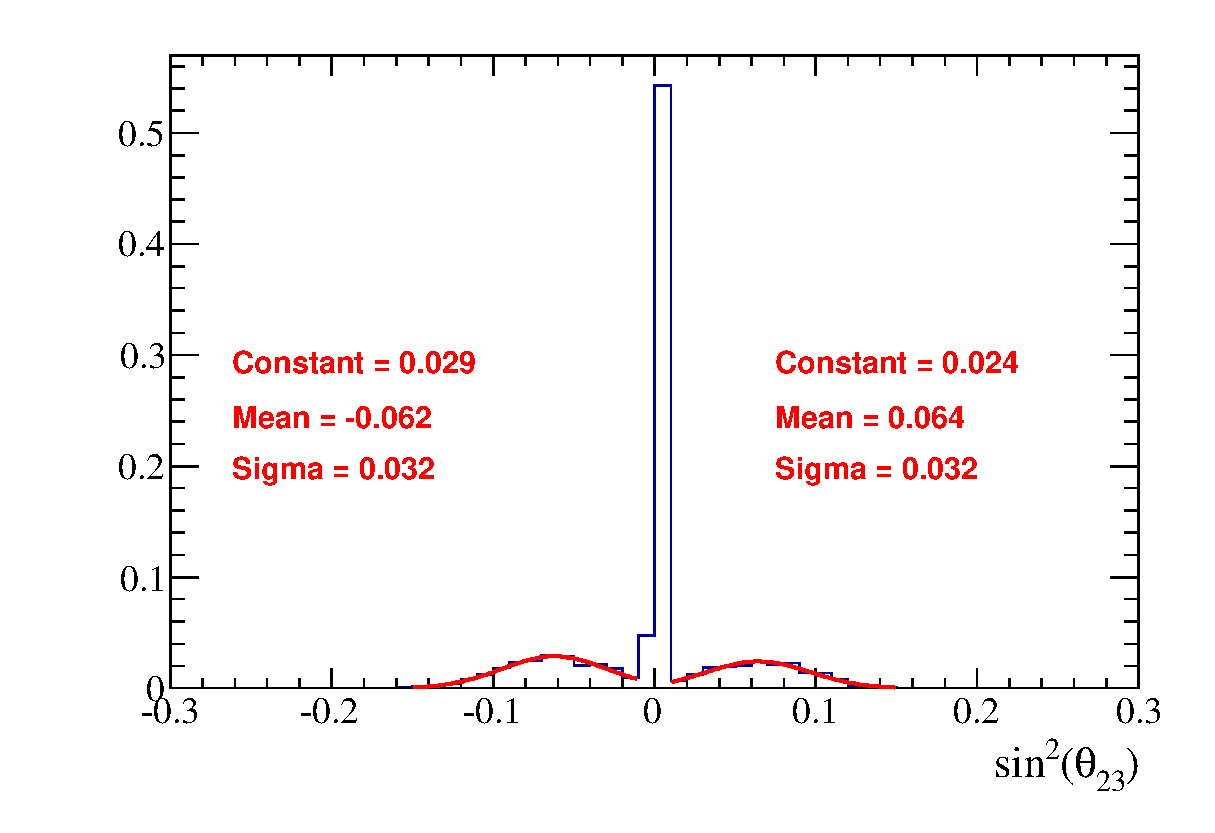
\includegraphics[width=20pc]{./images/fit_bias/Residuals_3peaks.eps}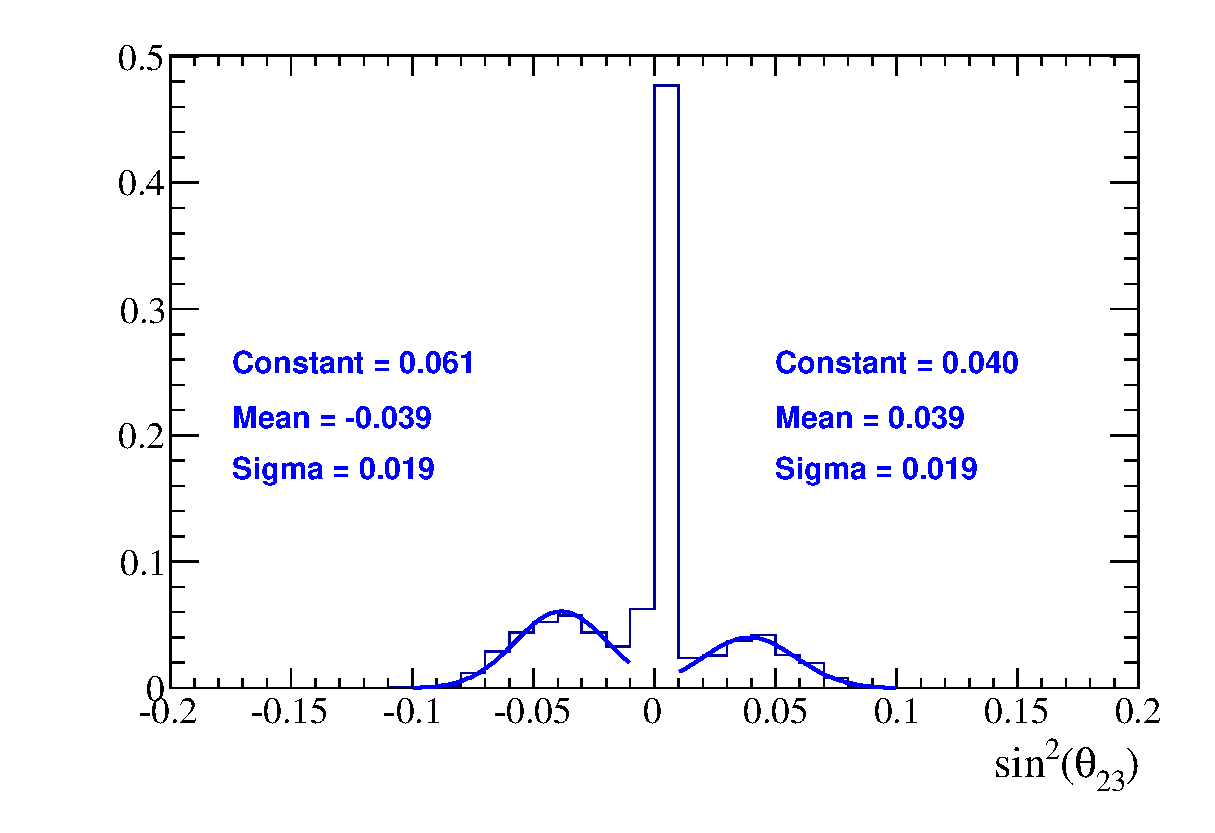
\includegraphics[width=20pc]{./images/fit_bias/Residuals_3peaks_goal.eps}
  \caption {
    Distributions of fitter residuals for $\sin^{2}\theta_{23}$ for 5k toy MC experiments,
    generated at $\sin^{2}\theta_{23}$ = 0.513 and
    $|\Delta m^{2}_{32}|$ = 2.4$\times$10$^{-3}$ eV$^{2}$/c$^{4}$,
    including statistical fluctuations and with randomized systematic and non-23 oscillation parameters,
    stressing the three-peak structure and including a Gaussian fit for the extra peaks at non-maximal disappearance.
    The distribution is shown for both
    6.5700$\times$10$^{20}$ POT (Run 1+2+3+4, left plot) and 7.8$\times$10$^{21}$ POT (the T2K ultimate goal, right plot).
  }
  \label{fig:residuals:3peaks}
\end{figure*}

\begin{table}[htbp]
\center
\begin{tabular}{|p{1.5cm}|p{2.5cm}|p{1.5cm}|p{1cm}|p{1.6cm}|p{1.6cm}|p{1.6cm}|p{1.6cm}|}
\hline
POT &   & Number  & Ratio &  \multicolumn{2}{c|}{Input value of $\sin^{2}\theta_{23}$} & \multicolumn{2}{c|}{Peak of} \\
& & of events & osc/        & \multicolumn{2}{c|}{giving this ratio}   & \multicolumn{2}{c|}{non-maximal fitted} \\
  & &  & no osc        &   \multicolumn{2}{c|}{osc/no osc}  & \multicolumn{2}{c|}{values of $\sin^{2}\theta_{23}$} \\
\cline{5-8}
   & &  &         & (Octant 1) & (Octant 2) & (Octant 1) & (Octant 2) \\
\hline \hline
\multirow{3}{*}{6.57$\times$10$^{20}$} & No oscillations  & 37.934 & 1 & & & \multirow{3}{*}{0.451} & \multirow{3}{*}{0.577} \\
\cline{2-6}
 & $\sin^{2}\theta_{23}$ = 0.513 (no fluctuation) & 2.672 & 0.070 & & & & \\
\cline{2-6}
 & $\sin^{2}\theta_{23}$ = 0.513 (fluctuation 1) & 3 & 0.079 & 0.463 & 0.565 & & \\
\hline \hline
\multirow{7}{*}{7.8$\times$10$^{21}$} & No oscillations & 450.352 & 1 & & & \multirow{7}{*}{0.474} & \multirow{7}{*}{0.552} \\
\cline{2-6}
 & $\sin^{2}\theta_{23}$ = 0.513 (no fluctuation) & 31.545 & 0.070 & & & & \\
\cline{2-6}
 & $\sin^{2}\theta_{23}$ = 0.513 (fluctuation 1)  & 32 & 0.071 & 0.497 & 0.531 &  &  \\
\cline{2-6}
 & $\sin^{2}\theta_{23}$ = 0.513 (fluctuation 2)  & 33 & 0.073 & 0.484 & 0.544 &  &  \\
\cline{2-6}
 &$\sin^{2}\theta_{23}$ = 0.513 (fluctuation 3) & 34 & 0.075 & 0.474 & 0.553 &  &  \\
\cline{2-6}
 &$\sin^{2}\theta_{23}$ = 0.513 (fluctuation 4) & 35 & 0.078 & 0.467 & 0.561 &  & \\
\cline{2-6}
 &$\sin^{2}\theta_{23}$ = 0.513 (fluctuation 5) & 36 & 0.080 & 0.461 & 0.566 &  & \\
\hline
\end{tabular}
\caption{
Numbers of events in a single bin at the lowest part of the oscillation dip with oscillations and ratio to number without oscillations for a true input 
value $\sin^{2}\theta_{23}$ = 0.513 at 6.57$\times$10$^{20}$ POT (Run 1+2+3+4) and 7.8$\times$10$^{21}$ POT (the ultimate T2K goal). These numbers are 
shown without statistical fluctuations and with different upward fluctuations. Also shown are the input values of $\sin^{2}\theta_{23}$ to toy datasets 
from Fig.\ \ref{fig:residuals:ratio_at_minimum} matching the ratio of number of events with oscillations to number without oscillations. These values of 
$\sin^{2}\theta_{23}$ can be compared with the peaks of the non-maximal fitted values of $\sin^{2}\theta_{23}$ from the Gaussian fits in Fig.\ 
\ref{fig:residuals:3peaks}.}
\label{tab:residuals:3peaks}
\end{table}

\begin{figure*}[htb]
  \center
  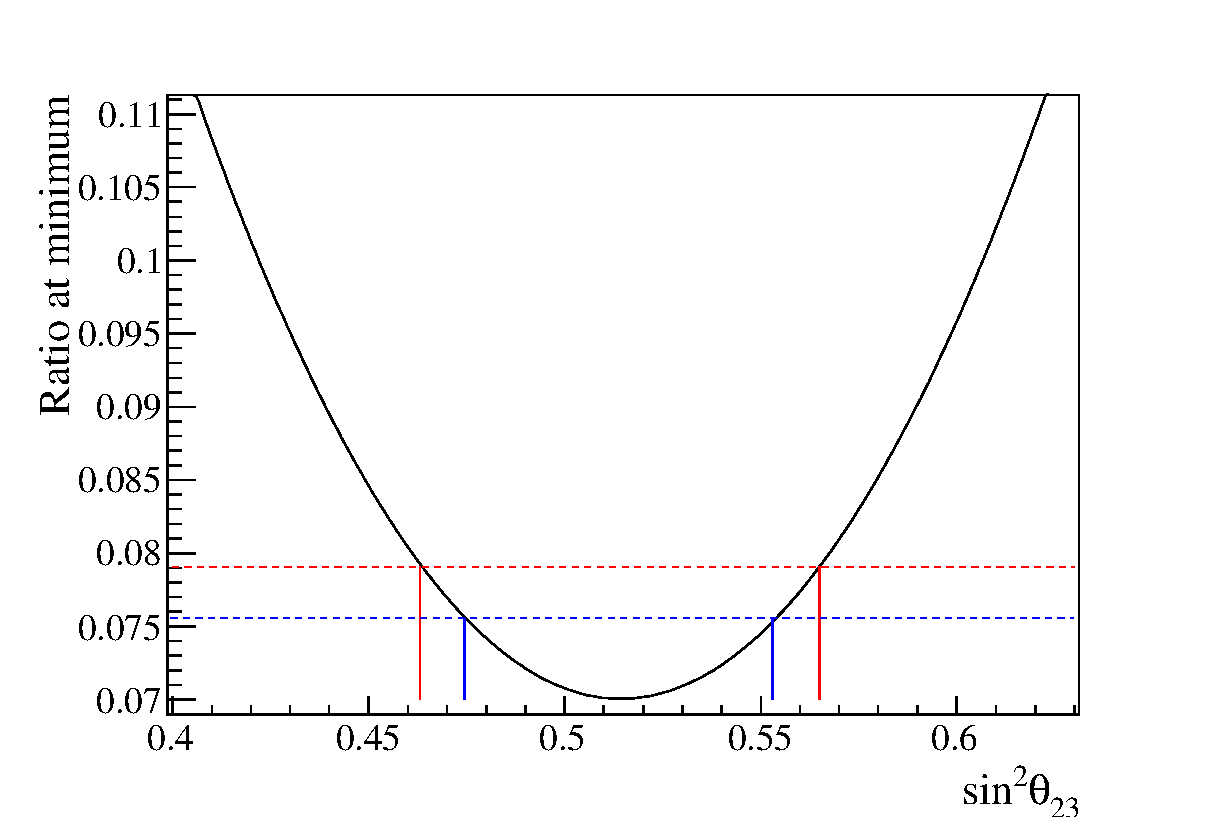
\includegraphics[width=25pc]{./images/fit_bias/Ratio_at_minimum.eps}
  \caption {
    Ratio of number of events in a single bin at the lowest part of the oscillation dip for toy datasets
    created with different input values of $\sin^{2}\theta_{23}$ to number without oscillations
    against the input value of $\sin^{2}\theta_{23}$. Red (blue) lines show the value corresponding to
    the ratio found at 6.5700$\times$10$^{20}$ POT (7.8$\times$10$^{21}$ POT, the T2K ultimate POT goal)
    in Fig.\ \ref{fig:residuals:3peaks}.
  }
  \label{fig:residuals:ratio_at_minimum}
\end{figure*}


%\begin{figure*}[htb]
%  \center
%  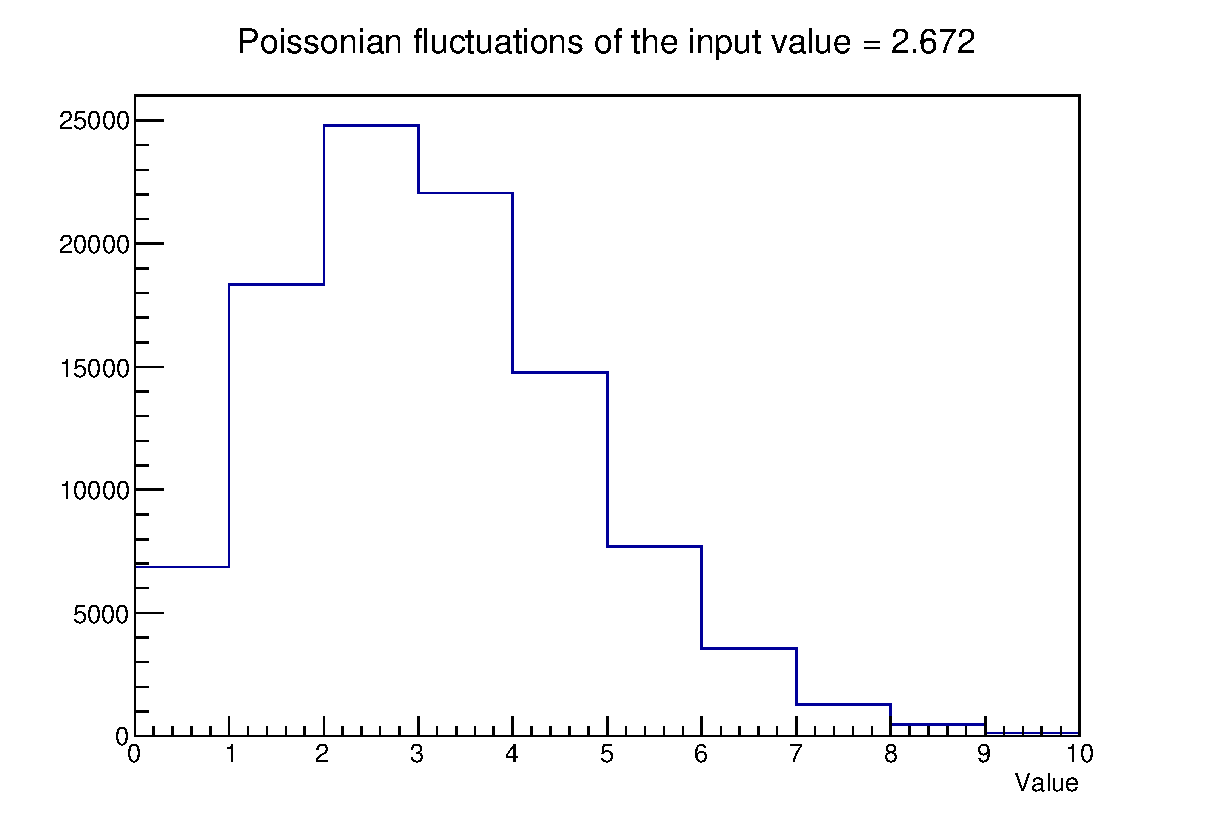
\includegraphics[width=20pc]{./images/fit_bias/Poisson_fluct_dip.eps}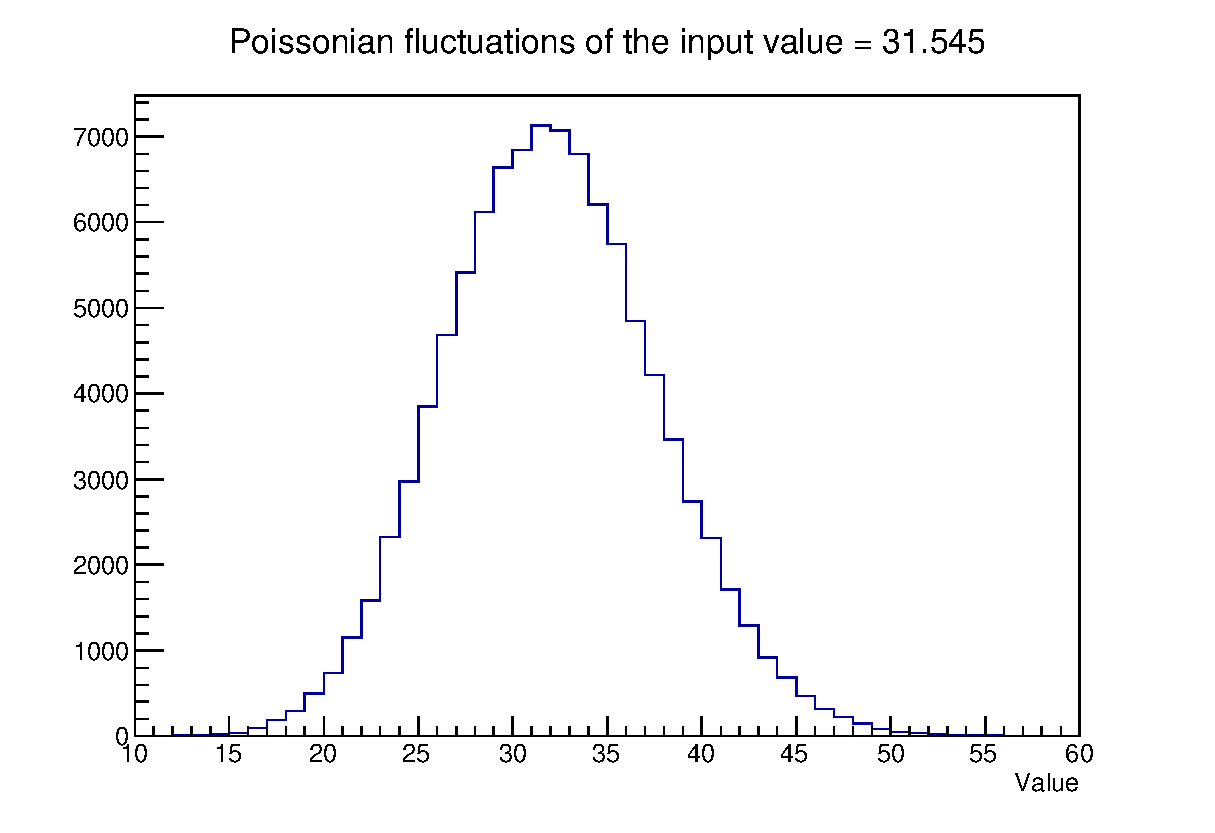
\includegraphics[width=20pc]{./images/fit_bias/Poisson_fluct_dip_goal.eps}
%  \caption {
%    Distributions of 100k Poisson fluctuations of the number of
%    events in a single bin at the lowest part of the oscillation dip for an input value of $\sin^{2}\theta_{23}$ = 0.513
%    These distributions are shown for means of 2.672 events (for 6.5700$\times$10$^{20}$ POT, left plot) and 31.545 events
%    (for 7.8$\times$10$^{21}$ POT, the T2K ultimate POT goal, right plot).
%  }
%  \label{fig:residuals:poisson_fluct}
%\end{figure*}



%
% Systematic pull & summary plots
%
\begin{figure*}[htb]
  \center
  \includegraphics[width=40pc]{{./images/fit_bias/nuis_sys_0.002400_0.370_allpulls}.eps}
  \caption {
    Systematic pull distributions for all systematic parameters for
    5k toy MC experiments at 6.5700$\times$10$^{20}$ POT 
    generated at $\sin^{2}\theta_{23}$ = 0.370 and
    $|\Delta m^{2}_{32}|$ = 2.4$\times$10$^{-3}$ eV$^{2}$/c$^{4}$,
    including statistical fluctuations and with randomized systematic parameters.
    A Gaussian distribution of mean 0, width 1 is shown for reference.
    The two parameters that do not have a Gaussian distribution are $\delta_{CP}$ and $f_{SF; t, r}$.
  }
  \label{fig:pulls:syst:0.370}
\end{figure*}

\begin{figure*}[htb]
  \center
  \includegraphics[width=50pc,angle=270]{{./images/fit_bias/nuis_sys_0.002400_0.370_bigsummary}.eps}
  \caption {
    Summary of systematic pull distributions for all systematic parameters for
    5k toy MC experiments at 6.5700$\times$10$^{20}$ POT 
    generated at $\sin^{2}\theta_{23}$ = 0.370 and
    $|\Delta m^{2}_{32}|$ = 2.4$\times$10$^{-3}$ eV$^{2}$/c$^{4}$,
    including statistical fluctuations and with randomized systematic parameters.
    The tests shown are the mean, RMS, skewness and kurtosis.
    % and the p-value from 
    % a Kolmogorov-Smirnov test comparing the pull distribution with a normal distribution of
    % mean 0, width 1.
  }
  \label{fig:pulls:syst:summary:0.370}
\end{figure*}

\begin{figure*}[htb]
  \center
  \includegraphics[width=38pc]{{./images/fit_bias/nuis_sys_0.002400_0.370_importpull_1_5}.eps}
  \caption {
    Pull distributions for $\delta_{CP}$,
    $f_{SF; t, r}$,
    $f_{\pi-less\Delta; t, r}$,
    $f_{E; r}^{SK}$,
    and $f_{i; r}^{SK+FSI}$,
    computed from fits of 5k toy MC experiments at 
    6.5700$\times$10$^{20}$ POT, generated at $\sin^{2}\theta_{23}$ = 0.370 and
    $|\Delta m^{2}_{32}|$ = 2.4$\times$10$^{-3}$ eV$^{2}$/c$^{4}$,
    including statistical fluctuations and with randomized systematic parameters.
  }
  \label{fig:pulls:syst:important:0.370}
\end{figure*}

\begin{figure*}[htb]
  \center
  \includegraphics[width=40pc]{{./images/fit_bias/nuis_sys_0.002400_0.650_allpulls}.eps}
  \caption {
    Systematic pull distributions for all systematic parameters for
    5k toy MC experiments at 6.5700$\times$10$^{20}$ POT 
    generated at $\sin^{2}\theta_{23}$ = 0.650 and
    $|\Delta m^{2}_{32}|$ = 2.4$\times$10$^{-3}$ eV$^{2}$/c$^{4}$,
    including statistical fluctuations and with randomized systematic parameters.
    A Gaussian distribution of mean 0, width 1 is shown for reference.
    The two non-Gaussian parameters are $\delta_{CP}$ and $f_{SF; t, r}$.
  }
  \label{fig:pulls:syst:0.650}
\end{figure*}

\begin{figure*}[htb]
  \center
  \includegraphics[width=50pc,angle=270]{{./images/fit_bias/nuis_sys_0.002400_0.650_bigsummary}.eps}
  \caption {
    Summary of systematic pull distributions for all systematic parameters for
    5k toy MC experiments at 6.5700$\times$10$^{20}$ POT 
    generated at $\sin^{2}\theta_{23}$ = 0.650 and
    $|\Delta m^{2}_{32}|$ = 2.4$\times$10$^{-3}$ eV$^{2}$/c$^{4}$,
    including statistical fluctuations and with randomized systematic parameters.
    The tests shown are the mean, RMS, skewness and kurtosis.
    % and the p-value from 
    % a Kolmogorov-Smirnov test comparing the pull distribution with a normal distribution of
    % mean 0, width 1.
  }
  \label{fig:pulls:syst:summary:0.650}
\end{figure*}

\begin{figure*}[htb]
  \center
  \includegraphics[width=38pc]{{./images/fit_bias/nuis_sys_0.002400_0.650_importpull_1_5}.eps}
  \caption {
    Pull distributions for $\delta_{CP}$,
    $f_{SF; t, r}$,
    $f_{\pi-less\Delta; t, r}$,
    $f_{E; r}^{SK}$,
    and $f_{i; r}^{SK+FSI}$,
    computed from fits of 5k toy MC experiments at 
    6.5700$\times$10$^{20}$ POT, generated at $\sin^{2}\theta_{23}$ = 0.650 and
    $|\Delta m^{2}_{32}|$ = 2.4$\times$10$^{-3}$ eV$^{2}$/c$^{4}$,
    including statistical fluctuations and with randomized systematic parameters.
  }
  \label{fig:pulls:syst:important:0.650}
\end{figure*}

\begin{figure*}[htb]
  \center
  \includegraphics[width=40pc]{{./images/fit_bias/nuis_sys_0.002400_0.513_allpulls}.eps}
  \caption {
    Systematic pull distributions for all systematic parameters for
    5k toy MC experiments at 6.5700$\times$10$^{20}$ POT 
    generated at $\sin^{2}\theta_{23}$ = 0.513 and
    $|\Delta m^{2}_{32}|$ = 2.4$\times$10$^{-3}$ eV$^{2}$/c$^{4}$,
    including statistical fluctuations and with randomized systematic parameters.
    A Gaussian distribution of mean 0, width 1 is shown for reference.
    The two non-Gaussian parameters are $\delta_{CP}$ and $f_{SF; t, r}$.
  }
  \label{fig:pulls:syst:0.513}
\end{figure*}

\begin{figure*}[htb]
  \center
  \includegraphics[width=50pc,angle=270]{{./images/fit_bias/nuis_sys_0.002400_0.513_bigsummary}.eps}
  \caption {
    Summary of systematic pull distributions for all systematic parameters for
    5k toy MC experiments at 6.5700$\times$10$^{20}$ POT 
    generated at $\sin^{2}\theta_{23}$ = 0.513 and
    $|\Delta m^{2}_{32}|$ = 2.4$\times$10$^{-3}$ eV$^{2}$/c$^{4}$,
    including statistical fluctuations and with randomized systematic parameters.
    The tests shown are the mean, RMS, skewness and kurtosis.
    % and the p-value from 
    % a Kolmogorov-Smirnov test comparing the pull distribution with a normal distribution of
    % mean 0, width 1.
  }
  \label{fig:pulls:syst:summary:0.513}
\end{figure*}

\begin{figure*}[htb]
  \center
  \includegraphics[width=38pc]{{./images/fit_bias/nuis_sys_0.002400_0.513_importpull_1_5}.eps}
  \caption {
    Pull distributions for $\delta_{CP}$,
    $f_{SF; t, r}$,
    $f_{\pi-less\Delta; t, r}$,
    $f_{E; r}^{SK}$,
    and $f_{i; r}^{SK+FSI}$,
    computed from fits of 5k toy MC experiments at 
    6.5700$\times$10$^{20}$ POT, generated at $\sin^{2}\theta_{23}$ = 0.513 and
    $|\Delta m^{2}_{32}|$ = 2.4$\times$10$^{-3}$ eV$^{2}$/c$^{4}$,
    including statistical fluctuations and with randomized systematic parameters.
  }
  \label{fig:pulls:syst:important:0.513}
\end{figure*}



% these have been replaced with the same information, just combining
% current & future POT
% %
% % Osc param residuals for 0.37
% %
% \begin{figure*}[htb]
% \begin{minipage}[t]{0.48\linewidth}
% \center
% \includegraphics[width=20pc]{{./images/fit_bias/nuis_sys_0.002400_0.370_residual_0}.eps}
% \caption {
%   Residual distributions for $\sin^{2}\theta_{23}$ and $|\Delta m^2_{32}|$ 5k toy MC experiments at 
%   6.5700$\times$10$^{20}$ POT, generated at $\sin^{2}\theta_{23}$ = 0.370 and
%   $|\Delta m^{2}_{32}|$ = 2.4$\times$10$^{-3}$ eV$^{2}$/c$^{4}$,
%   including statistical fluctuations and with randomized systematic parameters.
% }
% \label{fig:syst_residuals:oscparam:run1234:0.370}
% \end{minipage}
% \hspace{0.06\linewidth}
% \begin{minipage}[t]{0.48\linewidth}
% \center
% \includegraphics[width=20pc]{{./images/fit_bias/nuis_sys_0.002400_0.370_goalpot_residual_0}.eps}
% \caption {
%   Residual distributions for $\sin^{2}\theta_{23}$ and $|\Delta m^2_{32}|$ 5k toy MC experiments at 
%   7.8$\times$10$^{21}$ POT (the T2K ultimate POT goal), generated at $\sin^{2}\theta_{23}$ = 0.370 and
%   $|\Delta m^{2}_{32}|$ = 2.4$\times$10$^{-3}$ eV$^{2}$/c$^{4}$,
%   including statistical fluctuations and with randomized systematic parameters.
% }
% \label{fig:syst_residuals:oscparam:potgoal:0.370}
% \end{minipage}
% \end{figure*}

% %
% % Osc param residuals for 0.65
% %
% \begin{figure*}[htb]
% \begin{minipage}[t]{0.48\linewidth}
% \center
% \includegraphics[width=20pc]{{./images/fit_bias/nuis_sys_0.002400_0.650_residual_0}.eps}
% \caption {
%   Residual distributions for $\sin^{2}\theta_{23}$ and $|\Delta m^2_{32}|$ 5k toy MC experiments at 
%   6.5700$\times$10$^{20}$ POT, generated at $\sin^{2}\theta_{23}$ = 0.650 and
%   $|\Delta m^{2}_{32}|$ = 2.4$\times$10$^{-3}$ eV$^{2}$/c$^{4}$,
%   including statistical fluctuations and with randomized systematic parameters.
% }
% \label{fig:syst_residuals:oscparam:run1234:0.650}
% \end{minipage}
% \hspace{0.06\linewidth}
% \begin{minipage}[t]{0.48\linewidth}
% \center
% \includegraphics[width=20pc]{{./images/fit_bias/nuis_sys_0.002400_0.650_goalpot_residual_0}.eps}
% \caption {
%   Residual distributions for $\sin^{2}\theta_{23}$ and $|\Delta m^2_{32}|$ 5k toy MC experiments at 
%   7.8$\times$10$^{21}$ POT (the T2K ultimate POT goal), generated at $\sin^{2}\theta_{23}$ = 0.650 and
%   $|\Delta m^{2}_{32}|$ = 2.4$\times$10$^{-3}$ eV$^{2}$/c$^{4}$,
%   including statistical fluctuations and with randomized systematic parameters.
% }
% \label{fig:syst_residuals:oscparam:potgoal:0.650}
% \end{minipage}
% \end{figure*}

% %
% % Osc param residuals for 0.513
% %
% \begin{figure*}[htb]
% \begin{minipage}[t]{0.48\linewidth}
% \center
% \includegraphics[width=20pc]{{./images/fit_bias/nuis_sys_0.002400_0.513_residual_0}.eps}
% \caption {
%   Residual distributions for $\sin^{2}\theta_{23}$ and $|\Delta m^2_{32}|$ 5k toy MC experiments at 
%   6.5700$\times$10$^{20}$ POT, generated at $\sin^{2}\theta_{23}$ = 0.513 and
%   $|\Delta m^{2}_{32}|$ = 2.4$\times$10$^{-3}$ eV$^{2}$/c$^{4}$,
%   including statistical fluctuations and with randomized systematic parameters.
% }
% \label{fig:syst_residuals:oscparam:run1234:0.513}
% \end{minipage}
% \hspace{0.06\linewidth}
% \begin{minipage}[t]{0.48\linewidth}
% \center
% \includegraphics[width=20pc]{{./images/fit_bias/nuis_sys_0.002400_0.513_goalpot_residual_0}.eps}
% \caption {
%   Residual distributions for $\sin^{2}\theta_{23}$ and $|\Delta m^2_{32}|$ 5k toy MC experiments at 
%   7.8$\times$10$^{21}$ POT (the T2K ultimate POT goal), generated at $\sin^{2}\theta_{23}$ = 0.513 and
%   $|\Delta m^{2}_{32}|$ = 2.4$\times$10$^{-3}$ eV$^{2}$/c$^{4}$,
%   including statistical fluctuations and with randomized systematic parameters.
% }
% \label{fig:syst_residuals:oscparam:potgoal:0.513}
% \end{minipage}
% \end{figure*}

%these have been replaced with the 'all' plot, 'summary' plot and the 'important' plot
%
% Systematic residuals for 0.37
%
% \begin{figure*}[htb]
% \begin{minipage}[t]{0.48\linewidth}
% \center
% \includegraphics[width=20pc]{{./images/fit_bias/nuis_sys_0.002400_0.370_residual_1}.eps}
% \caption {
%   Residual distributions for $\sin^{2}\theta_{13}$, $\sin^{2}\theta_{12}$, $\Delta m^2_{21}$,
%   and $f_{0; t, r}^{banff}$-$f_{8; t, r}^{banff}$,
%   computed from fits of 5k toy MC experiments at 
%   6.5700$\times$10$^{20}$ POT, generated at $\sin^{2}\theta_{23}$ = 0.370 and
%   $|\Delta m^{2}_{32}|$ = 2.4$\times$10$^{-3}$ eV$^{2}$/c$^{4}$,
%   including statistical fluctuations and with randomized systematic parameters.
% }
% \label{fig:syst_residuals1:run1234:0.370}
% \end{minipage}
% \hspace{0.06\linewidth}
% \begin{minipage}[t]{0.48\linewidth}
% \center
% \includegraphics[width=20pc]{{./images/fit_bias/nuis_sys_0.002400_0.370_residual_2}.eps}
% \caption {
%   Residual distributions for
%   $f_{9; t, r}^{banff}$-$f_{20; t, r}^{banff}$,
%   computed from fits of 5k toy MC experiments at 
%   6.5700$\times$10$^{20}$ POT, generated at $\sin^{2}\theta_{23}$ = 0.370 and
%   $|\Delta m^{2}_{32}|$ = 2.4$\times$10$^{-3}$ eV$^{2}$/c$^{4}$,
%   including statistical fluctuations and with randomized systematic parameters.
% }
% \label{fig:syst_residuals2:run1234:0.370}
% \end{minipage}
% \vfill
% \begin{minipage}[t]{0.48\linewidth}
% \center
% \includegraphics[width=20pc]{{./images/fit_bias/nuis_sys_0.002400_0.370_residual_3}.eps}
% \caption {
%   Residual distributions for
%   $f_{21; t, r}^{banff}$-$f_{22; t, r}^{banff}$,
%   and the first 10 uncorrelated cross section parameters,
%   computed from fits of 5k toy MC experiments at 
%   6.5700$\times$10$^{20}$ POT, generated at $\sin^{2}\theta_{23}$ = 0.370 and
%   $|\Delta m^{2}_{32}|$ = 2.4$\times$10$^{-3}$ eV$^{2}$/c$^{4}$,
%   including statistical fluctuations and with randomized systematic parameters.
% }
% \label{fig:syst_residuals3:run1234:0.370}
% \end{minipage}
% \hspace{0.06\linewidth}
% \begin{minipage}[t]{0.48\linewidth}
% \center
% \includegraphics[width=20pc]{{./images/fit_bias/nuis_sys_0.002400_0.370_residual_4}.eps}
% \caption {
%   Residual distributions for
%   $f_{CC\bar{\nu}; t}$, $f_{E; r}^{SK}$, and $f _{0; r}^{SK+FSI}$-$f _{5; r}^{SK+FSI}$ 
%   computed from fits of 5k toy MC experiments at 
%   6.5700$\times$10$^{20}$ POT, generated at $\sin^{2}\theta_{23}$ = 0.370 and
%   $|\Delta m^{2}_{32}|$ = 2.4$\times$10$^{-3}$ eV$^{2}$/c$^{4}$,
%   including statistical fluctuations and with randomized systematic parameters.
% }
% \label{fig:syst_residuals4:run1234:0.370}
% \end{minipage}
% \end{figure*}

%
% Systematic pulls for 0.37
%
% \begin{figure*}[htb]
% \begin{minipage}[t]{0.48\linewidth}
% \center
% \includegraphics[width=20pc]{{./images/fit_bias/nuis_sys_0.002400_0.370_pull_1_1}.eps}
% \caption {
%   Pull distributions for $\sin^{2}\theta_{13}$, $\sin^{2}\theta_{12}$, $\Delta m^2_{21}$,
%   and $f_{0; t, r}^{banff}$-$f_{8; t, r}^{banff}$,
%   computed from fits of 5k toy MC experiments at 
%   6.5700$\times$10$^{20}$ POT, generated at $\sin^{2}\theta_{23}$ = 0.370 and
%   $|\Delta m^{2}_{32}|$ = 2.4$\times$10$^{-3}$ eV$^{2}$/c$^{4}$,
%   including statistical fluctuations and with randomized systematic parameters.
% }
% \label{fig:syst_pulls1:run1234:0.370}
% \end{minipage}
% \hspace{0.06\linewidth}
% \begin{minipage}[t]{0.48\linewidth}
% \center
% \includegraphics[width=20pc]{{./images/fit_bias/nuis_sys_0.002400_0.370_pull_1_2}.eps}
% \caption {
%   Pull distributions for
%   $f_{9; t, r}^{banff}$-$f_{20; t, r}^{banff}$,
%   computed from fits of 5k toy MC experiments at 
%   6.5700$\times$10$^{20}$ POT, generated at $\sin^{2}\theta_{23}$ = 0.370 and
%   $|\Delta m^{2}_{32}|$ = 2.4$\times$10$^{-3}$ eV$^{2}$/c$^{4}$,
%   including statistical fluctuations and with randomized systematic parameters.
% }
% \label{fig:syst_pulls2:run1234:0.370}
% \end{minipage}
% \vfill
% \begin{minipage}[t]{0.48\linewidth}
% \center
% \includegraphics[width=20pc]{{./images/fit_bias/nuis_sys_0.002400_0.370_pull_1_3}.eps}
% \caption {
%   Pull distributions for
%   $f_{21; t, r}^{banff}$-$f_{22; t, r}^{banff}$,
%   and the first 10 uncorrelated cross section parameters,
%   computed from fits of 5k toy MC experiments at 
%   6.5700$\times$10$^{20}$ POT, generated at $\sin^{2}\theta_{23}$ = 0.370 and
%   $|\Delta m^{2}_{32}|$ = 2.4$\times$10$^{-3}$ eV$^{2}$/c$^{4}$,
%   including statistical fluctuations and with randomized systematic parameters.
% }
% \label{fig:syst_pulls3:run1234:0.370}
% \end{minipage}
% \hspace{0.06\linewidth}
% \begin{minipage}[t]{0.48\linewidth}
% \center
% \includegraphics[width=20pc]{{./images/fit_bias/nuis_sys_0.002400_0.370_pull_1_4}.eps}
% \caption {
%   Pull distributions for
%   $f_{CC\bar{\nu}; t}$, $f_{E; r}^{SK}$, and $f _{0; r}^{SK+FSI}$-$f _{5; r}^{SK+FSI}$ 
%   computed from fits of 5k toy MC experiments at 
%   6.5700$\times$10$^{20}$ POT, generated at $\sin^{2}\theta_{23}$ = 0.370 and
%   $|\Delta m^{2}_{32}|$ = 2.4$\times$10$^{-3}$ eV$^{2}$/c$^{4}$,
%   including statistical fluctuations and with randomized systematic parameters.
% }
% \label{fig:syst_pulls4:run1234:0.370}
% \end{minipage}
% \end{figure*}


%
% Systematic residuals for 0.65
%
% \begin{figure*}[htb]
% \begin{minipage}[t]{0.48\linewidth}
% \center
% \includegraphics[width=20pc]{{./images/fit_bias/nuis_sys_0.002400_0.650_residual_1}.eps}
% \caption {
%   Residual distributions for $\sin^{2}\theta_{13}$, $\sin^{2}\theta_{12}$, $\Delta m^2_{21}$,
%   and $f_{0; t, r}^{banff}$-$f_{8; t, r}^{banff}$,
%   computed from fits of 5k toy MC experiments at 
%   6.5700$\times$10$^{20}$ POT, generated at $\sin^{2}\theta_{23}$ = 0.650 and
%   $|\Delta m^{2}_{32}|$ = 2.4$\times$10$^{-3}$ eV$^{2}$/c$^{4}$,
%   including statistical fluctuations and with randomized systematic parameters.
% }
% \label{fig:syst_residuals1:run1234:0.650}
% \end{minipage}
% \hspace{0.06\linewidth}
% \begin{minipage}[t]{0.48\linewidth}
% \center
% \includegraphics[width=20pc]{{./images/fit_bias/nuis_sys_0.002400_0.650_residual_2}.eps}
% \caption {
%   Residual distributions for
%   $f_{9; t, r}^{banff}$-$f_{20; t, r}^{banff}$,
%   computed from fits of 5k toy MC experiments at 
%   6.5700$\times$10$^{20}$ POT, generated at $\sin^{2}\theta_{23}$ = 0.650 and
%   $|\Delta m^{2}_{32}|$ = 2.4$\times$10$^{-3}$ eV$^{2}$/c$^{4}$,
%   including statistical fluctuations and with randomized systematic parameters.
% }
% \label{fig:syst_residuals2:run1234:0.650}
% \end{minipage}
% \vfill
% \begin{minipage}[t]{0.48\linewidth}
% \center
% \includegraphics[width=20pc]{{./images/fit_bias/nuis_sys_0.002400_0.650_residual_3}.eps}
% \caption {
%   Residual distributions for
%   $f_{21; t, r}^{banff}$-$f_{22; t, r}^{banff}$,
%   and the first 10 uncorrelated cross section parameters,
%   computed from fits of 5k toy MC experiments at 
%   6.5700$\times$10$^{20}$ POT, generated at $\sin^{2}\theta_{23}$ = 0.650 and
%   $|\Delta m^{2}_{32}|$ = 2.4$\times$10$^{-3}$ eV$^{2}$/c$^{4}$,
%   including statistical fluctuations and with randomized systematic parameters.
% }
% \label{fig:syst_residuals3:run1234:0.650}
% \end{minipage}
% \hspace{0.06\linewidth}
% \begin{minipage}[t]{0.48\linewidth}
% \center
% \includegraphics[width=20pc]{{./images/fit_bias/nuis_sys_0.002400_0.650_residual_4}.eps}
% \caption {
%   Residual distributions for
%   $f_{CC\bar{\nu}; t}$, $f_{E; r}^{SK}$, and $f _{0; r}^{SK+FSI}$-$f _{5; r}^{SK+FSI}$ 
%   computed from fits of 5k toy MC experiments at 
%   6.5700$\times$10$^{20}$ POT, generated at $\sin^{2}\theta_{23}$ = 0.650 and
%   $|\Delta m^{2}_{32}|$ = 2.4$\times$10$^{-3}$ eV$^{2}$/c$^{4}$,
%   including statistical fluctuations and with randomized systematic parameters.
% }
% \label{fig:syst_residuals4:run1234:0.650}
% \end{minipage}
% \end{figure*}

%
% Systematic pulls for 0.65
%
% \begin{figure*}[htb]
% \begin{minipage}[t]{0.48\linewidth}
% \center
% \includegraphics[width=20pc]{{./images/fit_bias/nuis_sys_0.002400_0.650_pull_1_1}.eps}
% \caption {
%   Pull distributions for $\sin^{2}\theta_{13}$, $\sin^{2}\theta_{12}$, $\Delta m^2_{21}$,
%   and $f_{0; t, r}^{banff}$-$f_{8; t, r}^{banff}$,
%   computed from fits of 5k toy MC experiments at 
%   6.5700$\times$10$^{20}$ POT, generated at $\sin^{2}\theta_{23}$ = 0.650 and
%   $|\Delta m^{2}_{32}|$ = 2.4$\times$10$^{-3}$ eV$^{2}$/c$^{4}$,
%   including statistical fluctuations and with randomized systematic parameters.
% }
% \label{fig:syst_pulls1:run1234:0.650}
% \end{minipage}
% \hspace{0.06\linewidth}
% \begin{minipage}[t]{0.48\linewidth}
% \center
% \includegraphics[width=20pc]{{./images/fit_bias/nuis_sys_0.002400_0.650_pull_1_2}.eps}
% \caption {
%   Pull distributions for
%   $f_{9; t, r}^{banff}$-$f_{20; t, r}^{banff}$,
%   computed from fits of 5k toy MC experiments at 
%   6.5700$\times$10$^{20}$ POT, generated at $\sin^{2}\theta_{23}$ = 0.650 and
%   $|\Delta m^{2}_{32}|$ = 2.4$\times$10$^{-3}$ eV$^{2}$/c$^{4}$,
%   including statistical fluctuations and with randomized systematic parameters.
% }
% \label{fig:syst_pulls2:run1234:0.650}
% \end{minipage}
% \vfill
% \begin{minipage}[t]{0.48\linewidth}
% \center
% \includegraphics[width=20pc]{{./images/fit_bias/nuis_sys_0.002400_0.650_pull_1_3}.eps}
% \caption {
%   Pull distributions for
%   $f_{21; t, r}^{banff}$-$f_{22; t, r}^{banff}$,
%   and the first 10 uncorrelated cross section parameters,
%   computed from fits of 5k toy MC experiments at 
%   6.5700$\times$10$^{20}$ POT, generated at $\sin^{2}\theta_{23}$ = 0.650 and
%   $|\Delta m^{2}_{32}|$ = 2.4$\times$10$^{-3}$ eV$^{2}$/c$^{4}$,
%   including statistical fluctuations and with randomized systematic parameters.
% }
% \label{fig:syst_pulls3:run1234:0.650}
% \end{minipage}
% \hspace{0.06\linewidth}
% \begin{minipage}[t]{0.48\linewidth}
% \center
% \includegraphics[width=20pc]{{./images/fit_bias/nuis_sys_0.002400_0.650_pull_1_4}.eps}
% \caption {
%   Pull distributions for
%   $f_{CC\bar{\nu}; t}$, $f_{E; r}^{SK}$, and $f _{0; r}^{SK+FSI}$-$f _{5; r}^{SK+FSI}$ 
%   computed from fits of 5k toy MC experiments at 
%   6.5700$\times$10$^{20}$ POT, generated at $\sin^{2}\theta_{23}$ = 0.650 and
%   $|\Delta m^{2}_{32}|$ = 2.4$\times$10$^{-3}$ eV$^{2}$/c$^{4}$,
%   including statistical fluctuations and with randomized systematic parameters.
% }
% \label{fig:syst_pulls4:run1234:0.650}
% \end{minipage}
% \end{figure*}


%
% Systematic residuals for 0.513
%
% \begin{figure*}[htb]
% \begin{minipage}[t]{0.48\linewidth}
% \center
% \includegraphics[width=20pc]{{./images/fit_bias/nuis_sys_0.002400_0.513_residual_1}.eps}
% \caption {
%   Residual distributions for $\sin^{2}\theta_{13}$, $\sin^{2}\theta_{12}$, $\Delta m^2_{21}$,
%   and $f_{0; t, r}^{banff}$-$f_{8; t, r}^{banff}$,
%   computed from fits of 5k toy MC experiments at 
%   6.5700$\times$10$^{20}$ POT, generated at $\sin^{2}\theta_{23}$ = 0.513 and
%   $|\Delta m^{2}_{32}|$ = 2.4$\times$10$^{-3}$ eV$^{2}$/c$^{4}$,
%   including statistical fluctuations and with randomized systematic parameters.
% }
% \label{fig:syst_residuals1:run1234:0.513}
% \end{minipage}
% \hspace{0.06\linewidth}
% \begin{minipage}[t]{0.48\linewidth}
% \center
% \includegraphics[width=20pc]{{./images/fit_bias/nuis_sys_0.002400_0.513_residual_2}.eps}
% \caption {
%   Residual distributions for
%   $f_{9; t, r}^{banff}$-$f_{20; t, r}^{banff}$,
%   computed from fits of 5k toy MC experiments at 
%   6.5700$\times$10$^{20}$ POT, generated at $\sin^{2}\theta_{23}$ = 0.513 and
%   $|\Delta m^{2}_{32}|$ = 2.4$\times$10$^{-3}$ eV$^{2}$/c$^{4}$,
%   including statistical fluctuations and with randomized systematic parameters.
% }
% \label{fig:syst_residuals2:run1234:0.513}
% \end{minipage}
% \vfill
% \begin{minipage}[t]{0.48\linewidth}
% \center
% \includegraphics[width=20pc]{{./images/fit_bias/nuis_sys_0.002400_0.513_residual_3}.eps}
% \caption {
%   Residual distributions for
%   $f_{21; t, r}^{banff}$-$f_{22; t, r}^{banff}$,
%   and the first 10 uncorrelated cross section parameters,
%   computed from fits of 5k toy MC experiments at 
%   6.5700$\times$10$^{20}$ POT, generated at $\sin^{2}\theta_{23}$ = 0.513 and
%   $|\Delta m^{2}_{32}|$ = 2.4$\times$10$^{-3}$ eV$^{2}$/c$^{4}$,
%   including statistical fluctuations and with randomized systematic parameters.
% }
% \label{fig:syst_residuals3:run1234:0.513}
% \end{minipage}
% \hspace{0.06\linewidth}
% \begin{minipage}[t]{0.48\linewidth}
% \center
% \includegraphics[width=20pc]{{./images/fit_bias/nuis_sys_0.002400_0.513_residual_4}.eps}
% \caption {
%   Residual distributions for
%   $f_{CC\bar{\nu}; t}$, $f_{E; r}^{SK}$, and $f _{0; r}^{SK+FSI}$-$f _{5; r}^{SK+FSI}$ 
%   computed from fits of 5k toy MC experiments at 
%   6.5700$\times$10$^{20}$ POT, generated at $\sin^{2}\theta_{23}$ = 0.513 and
%   $|\Delta m^{2}_{32}|$ = 2.4$\times$10$^{-3}$ eV$^{2}$/c$^{4}$,
%   including statistical fluctuations and with randomized systematic parameters.
% }
% \label{fig:syst_residuals4:run1234:0.513}
% \end{minipage}
% \end{figure*}

%
% Systematic pulls for 0.513
%
% \begin{figure*}[htb]
% \begin{minipage}[t]{0.48\linewidth}
% \center
% \includegraphics[width=20pc]{{./images/fit_bias/nuis_sys_0.002400_0.513_pull_1_1}.eps}
% \caption {
%   Pull distributions for $\sin^{2}\theta_{13}$, $\sin^{2}\theta_{12}$, $\Delta m^2_{21}$,
%   and $f_{0; t, r}^{banff}$-$f_{8; t, r}^{banff}$,
%   computed from fits of 5k toy MC experiments at 
%   6.5700$\times$10$^{20}$ POT, generated at $\sin^{2}\theta_{23}$ = 0.513 and
%   $|\Delta m^{2}_{32}|$ = 2.4$\times$10$^{-3}$ eV$^{2}$/c$^{4}$,
%   including statistical fluctuations and with randomized systematic parameters.
% }
% \label{fig:syst_pulls1:run1234:0.513}
% \end{minipage}
% \hspace{0.06\linewidth}
% \begin{minipage}[t]{0.48\linewidth}
% \center
% \includegraphics[width=20pc]{{./images/fit_bias/nuis_sys_0.002400_0.513_pull_1_2}.eps}
% \caption {
%   Pull distributions for
%   $f_{9; t, r}^{banff}$-$f_{20; t, r}^{banff}$,
%   computed from fits of 5k toy MC experiments at 
%   6.5700$\times$10$^{20}$ POT, generated at $\sin^{2}\theta_{23}$ = 0.513 and
%   $|\Delta m^{2}_{32}|$ = 2.4$\times$10$^{-3}$ eV$^{2}$/c$^{4}$,
%   including statistical fluctuations and with randomized systematic parameters.
% }
% \label{fig:syst_pulls2:run1234:0.513}
% \end{minipage}
% \vfill
% \begin{minipage}[t]{0.48\linewidth}
% \center
% \includegraphics[width=20pc]{{./images/fit_bias/nuis_sys_0.002400_0.513_pull_1_3}.eps}
% \caption {
%   Pull distributions for
%   $f_{21; t, r}^{banff}$-$f_{22; t, r}^{banff}$,
%   and the first 10 uncorrelated cross section parameters,
%   computed from fits of 5k toy MC experiments at 
%   6.5700$\times$10$^{20}$ POT, generated at $\sin^{2}\theta_{23}$ = 0.513 and
%   $|\Delta m^{2}_{32}|$ = 2.4$\times$10$^{-3}$ eV$^{2}$/c$^{4}$,
%   including statistical fluctuations and with randomized systematic parameters.
% }
% \label{fig:syst_pulls3:run1234:0.513}
% \end{minipage}
% \hspace{0.06\linewidth}
% \begin{minipage}[t]{0.48\linewidth}
% \center
% \includegraphics[width=20pc]{{./images/fit_bias/nuis_sys_0.002400_0.513_pull_1_4}.eps}
% \caption {
%   Pull distributions for
%   $f_{CC\bar{\nu}; t}$, $f_{E; r}^{SK}$, and $f _{0; r}^{SK+FSI}$-$f _{5; r}^{SK+FSI}$ 
%   computed from fits of 5k toy MC experiments at 
%   6.5700$\times$10$^{20}$ POT, generated at $\sin^{2}\theta_{23}$ = 0.513 and
%   $|\Delta m^{2}_{32}|$ = 2.4$\times$10$^{-3}$ eV$^{2}$/c$^{4}$,
%   including statistical fluctuations and with randomized systematic parameters.
% }
% \label{fig:syst_pulls4:run1234:0.513}
% \end{minipage}
% \end{figure*}

